\documentclass[11pt]{article}
\usepackage[textwidth=18.0cm, textheight=23.0cm, top=2.0cm]{geometry}
\usepackage{pst-all}
\usepackage{amssymb}
\usepackage{tikz}
\usepackage{underscore}\begin{document}
\pagestyle{empty}


ClassName: \underline{\textbf{Class_08.2bp-27}}
\par
BinSize: \underline{\textbf{100 × 100}}
\par
ReduceSize: \underline{\textbf{100 × 100}}
\par
TypeNum: \underline{\textbf{59}}
\par
Num: \underline{\textbf{60}}
\par
OutS: \underline{\textbf{170000}}
\par
InS: \underline{\textbf{146994}}
\par
Rate: \underline{\textbf{0.865}}
\par
UB: \underline{\textbf{17}}
\par
LB0: \underline{\textbf{17}}
\par
LB: \underline{\textbf{17}}
\par
LBWithCut: \underline{\textbf{17}}
\par
NodeCut: \underline{\textbf{0}}
\par
ExtendedNodeCnt: \underline{\textbf{1}}
\par
GenNodeCnt: \underline{\textbf{1}}
\par
PrimalNode: \underline{\textbf{0}}
\par
ColumnCount: \underline{\textbf{17}}
\par
TotalCutCount: \underline{\textbf{0}}
\par
RootCutCount: \underline{\textbf{0}}
\par
LPSolverCnt: \underline{\textbf{1}}
\par
PricingSolverCnt: \underline{\textbf{0}}
\par
BranchAndBoundNum: \underline{\textbf{1}}
\par
isOpt: \underline{\textbf{true}}
\par
TimeOnPrimal: \underline{\textbf{0.000 s}}
\par
TimeOnPricing: \underline{\textbf{0.000 s}}
\par
TimeOnRmp: \underline{\textbf{0.078 s}}
\par
TotalTime: \underline{\textbf{0.140 s}}
\par
\newpage


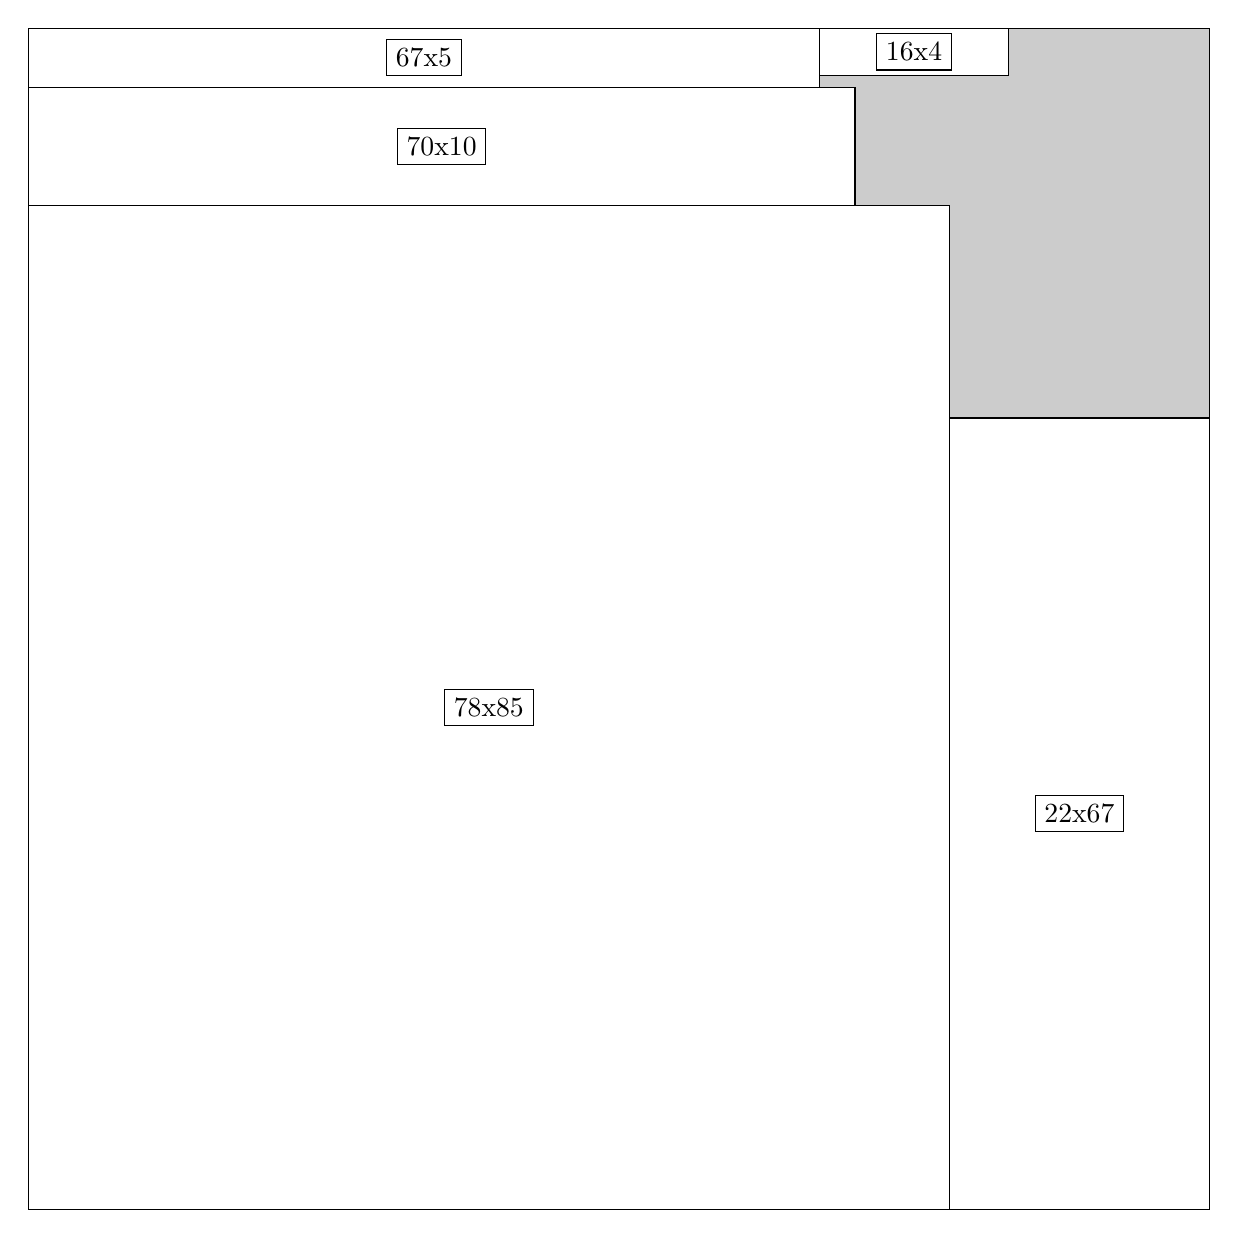
\begin{tikzpicture}[shorten >=1pt,scale=1.0,every node/.style={scale=1.0},->]
\tikzstyle{vertex}=[circle,fill=black!25,minimum size=14pt,inner sep=0pt]
\filldraw[fill=gray!40!white, draw=black] (0,0) rectangle (15.0,15.0);
\foreach \name/\x/\y/\w/\h in {78x85/0.0/0.0/11.7/12.75,22x67/11.7/0.0/3.3/10.049999999999999,70x10/0.0/12.75/10.5/1.5,67x5/0.0/14.25/10.049999999999999/0.75,16x4/10.049999999999999/14.399999999999999/2.4/0.6}
\filldraw[fill=white!40!white, draw=black] (\x,\y) rectangle node[draw] (\name) {\name} ++(\w,\h);
\end{tikzpicture}


w =78 , h =85 , x =0 , y =0 , v =6630
\par
w =22 , h =67 , x =78 , y =0 , v =1474
\par
w =70 , h =10 , x =0 , y =85 , v =700
\par
w =67 , h =5 , x =0 , y =95 , v =335
\par
w =16 , h =4 , x =67 , y =96 , v =64
\par
\newpage


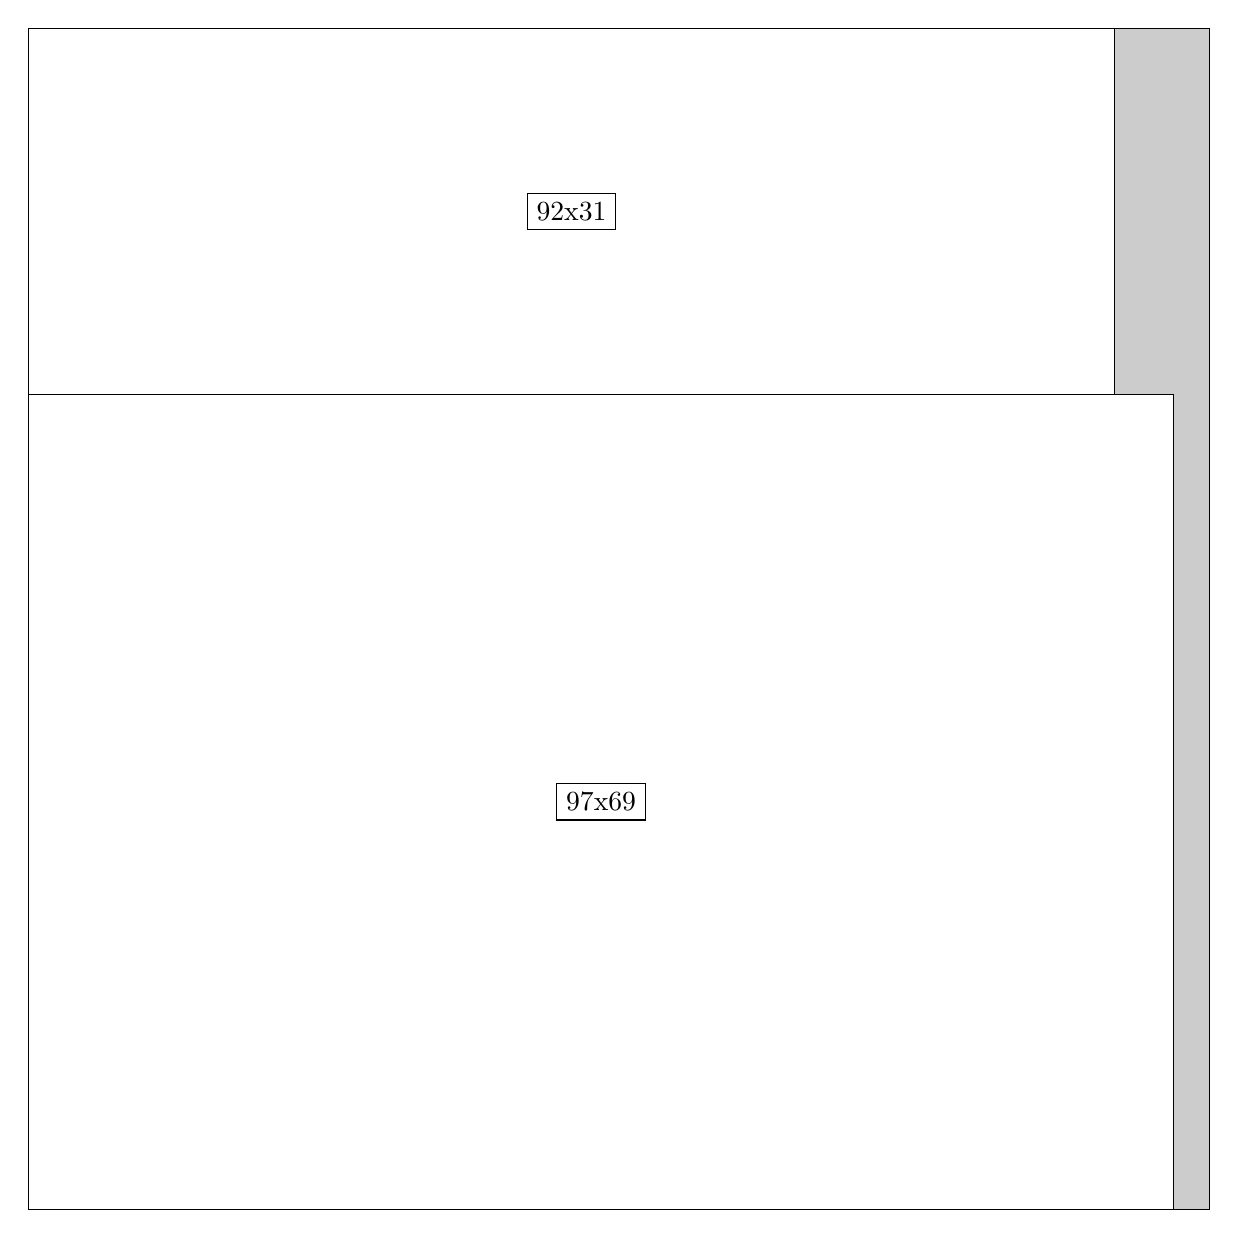
\begin{tikzpicture}[shorten >=1pt,scale=1.0,every node/.style={scale=1.0},->]
\tikzstyle{vertex}=[circle,fill=black!25,minimum size=14pt,inner sep=0pt]
\filldraw[fill=gray!40!white, draw=black] (0,0) rectangle (15.0,15.0);
\foreach \name/\x/\y/\w/\h in {97x69/0.0/0.0/14.549999999999999/10.35,92x31/0.0/10.35/13.799999999999999/4.6499999999999995}
\filldraw[fill=white!40!white, draw=black] (\x,\y) rectangle node[draw] (\name) {\name} ++(\w,\h);
\end{tikzpicture}


w =97 , h =69 , x =0 , y =0 , v =6693
\par
w =92 , h =31 , x =0 , y =69 , v =2852
\par
\newpage


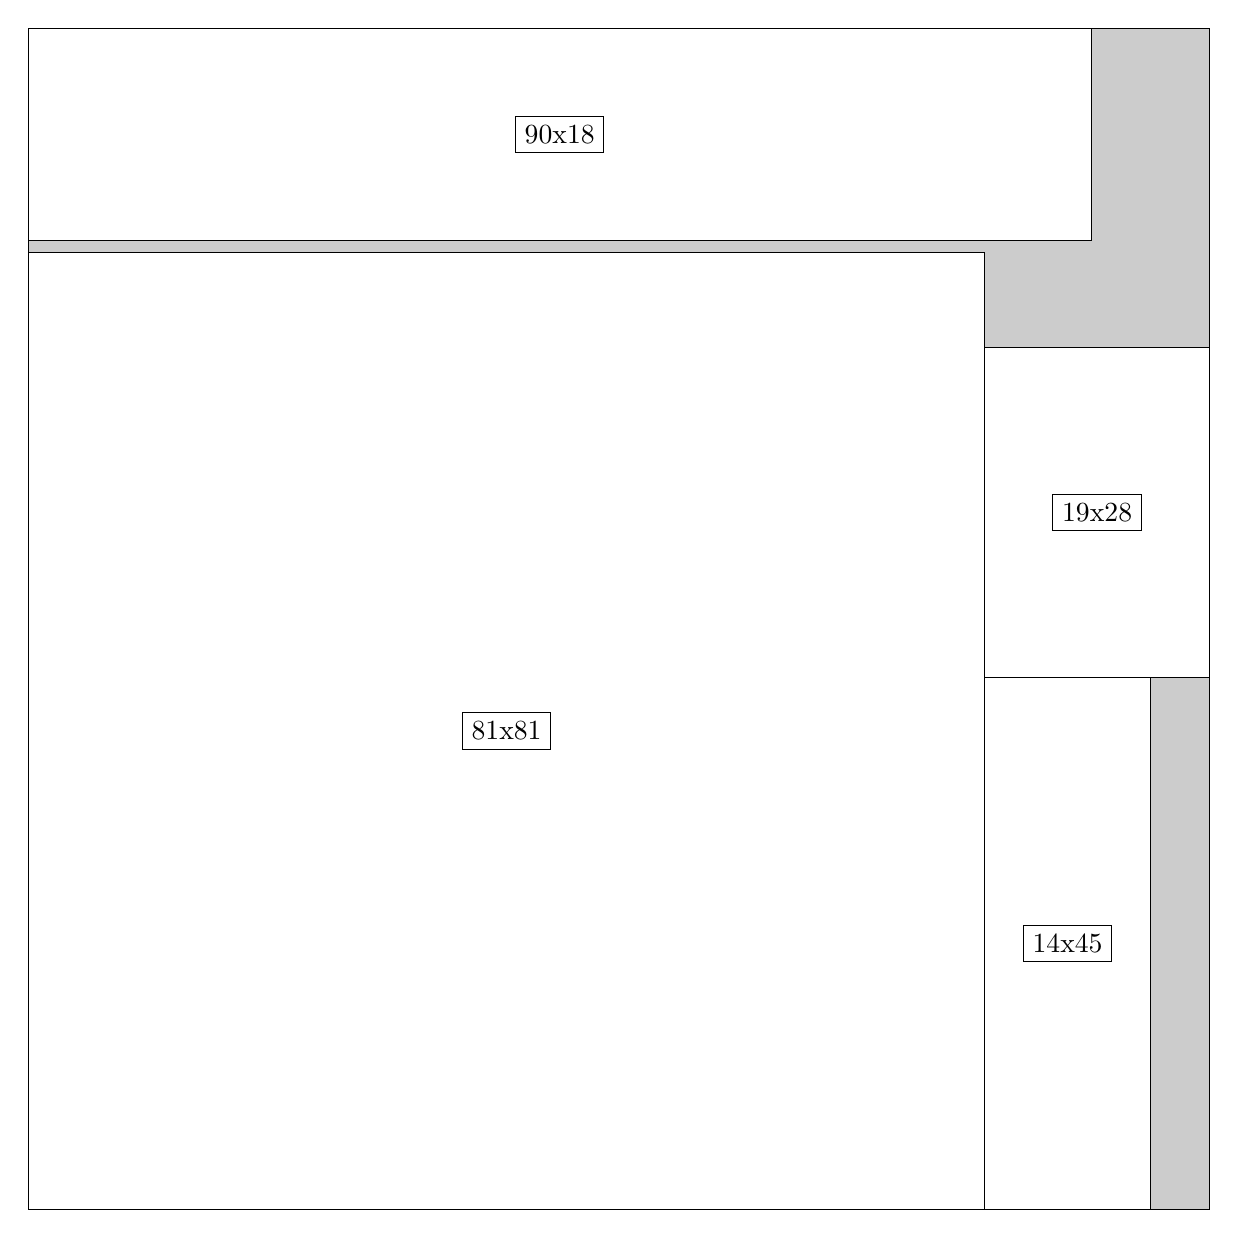
\begin{tikzpicture}[shorten >=1pt,scale=1.0,every node/.style={scale=1.0},->]
\tikzstyle{vertex}=[circle,fill=black!25,minimum size=14pt,inner sep=0pt]
\filldraw[fill=gray!40!white, draw=black] (0,0) rectangle (15.0,15.0);
\foreach \name/\x/\y/\w/\h in {81x81/0.0/0.0/12.15/12.15,90x18/0.0/12.299999999999999/13.5/2.6999999999999997,14x45/12.15/0.0/2.1/6.75,19x28/12.15/6.75/2.85/4.2}
\filldraw[fill=white!40!white, draw=black] (\x,\y) rectangle node[draw] (\name) {\name} ++(\w,\h);
\end{tikzpicture}


w =81 , h =81 , x =0 , y =0 , v =6561
\par
w =90 , h =18 , x =0 , y =82 , v =1620
\par
w =14 , h =45 , x =81 , y =0 , v =630
\par
w =19 , h =28 , x =81 , y =45 , v =532
\par
\newpage


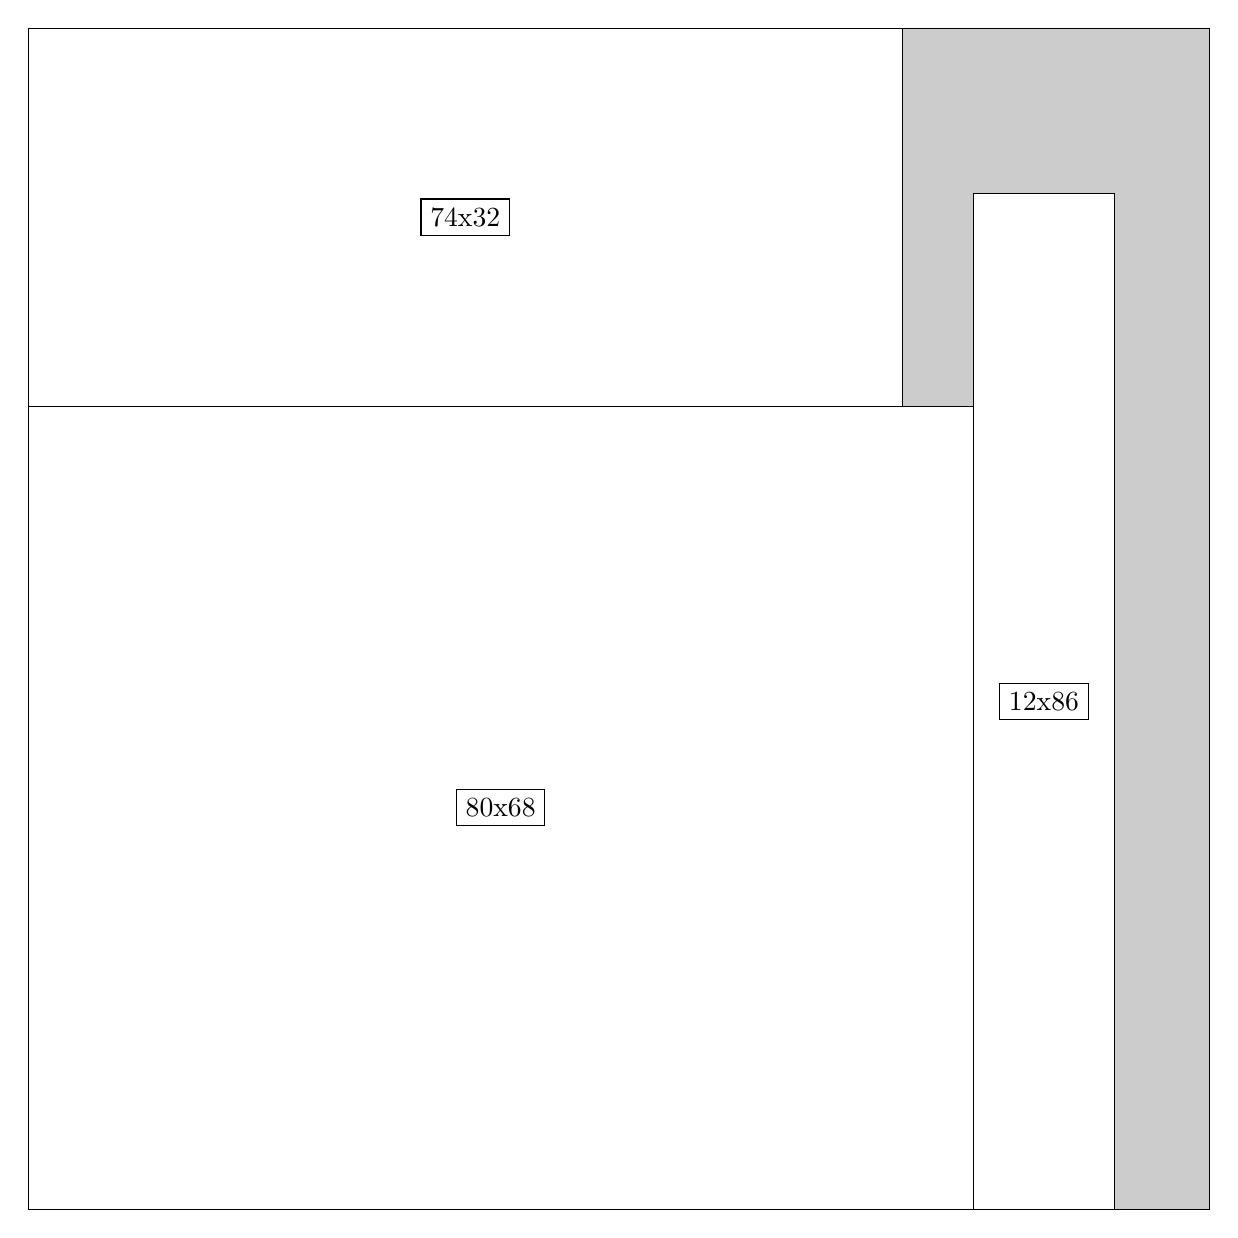
\begin{tikzpicture}[shorten >=1pt,scale=1.0,every node/.style={scale=1.0},->]
\tikzstyle{vertex}=[circle,fill=black!25,minimum size=14pt,inner sep=0pt]
\filldraw[fill=gray!40!white, draw=black] (0,0) rectangle (15.0,15.0);
\foreach \name/\x/\y/\w/\h in {80x68/0.0/0.0/12.0/10.2,74x32/0.0/10.2/11.1/4.8,12x86/12.0/0.0/1.7999999999999998/12.9}
\filldraw[fill=white!40!white, draw=black] (\x,\y) rectangle node[draw] (\name) {\name} ++(\w,\h);
\end{tikzpicture}


w =80 , h =68 , x =0 , y =0 , v =5440
\par
w =74 , h =32 , x =0 , y =68 , v =2368
\par
w =12 , h =86 , x =80 , y =0 , v =1032
\par
\newpage


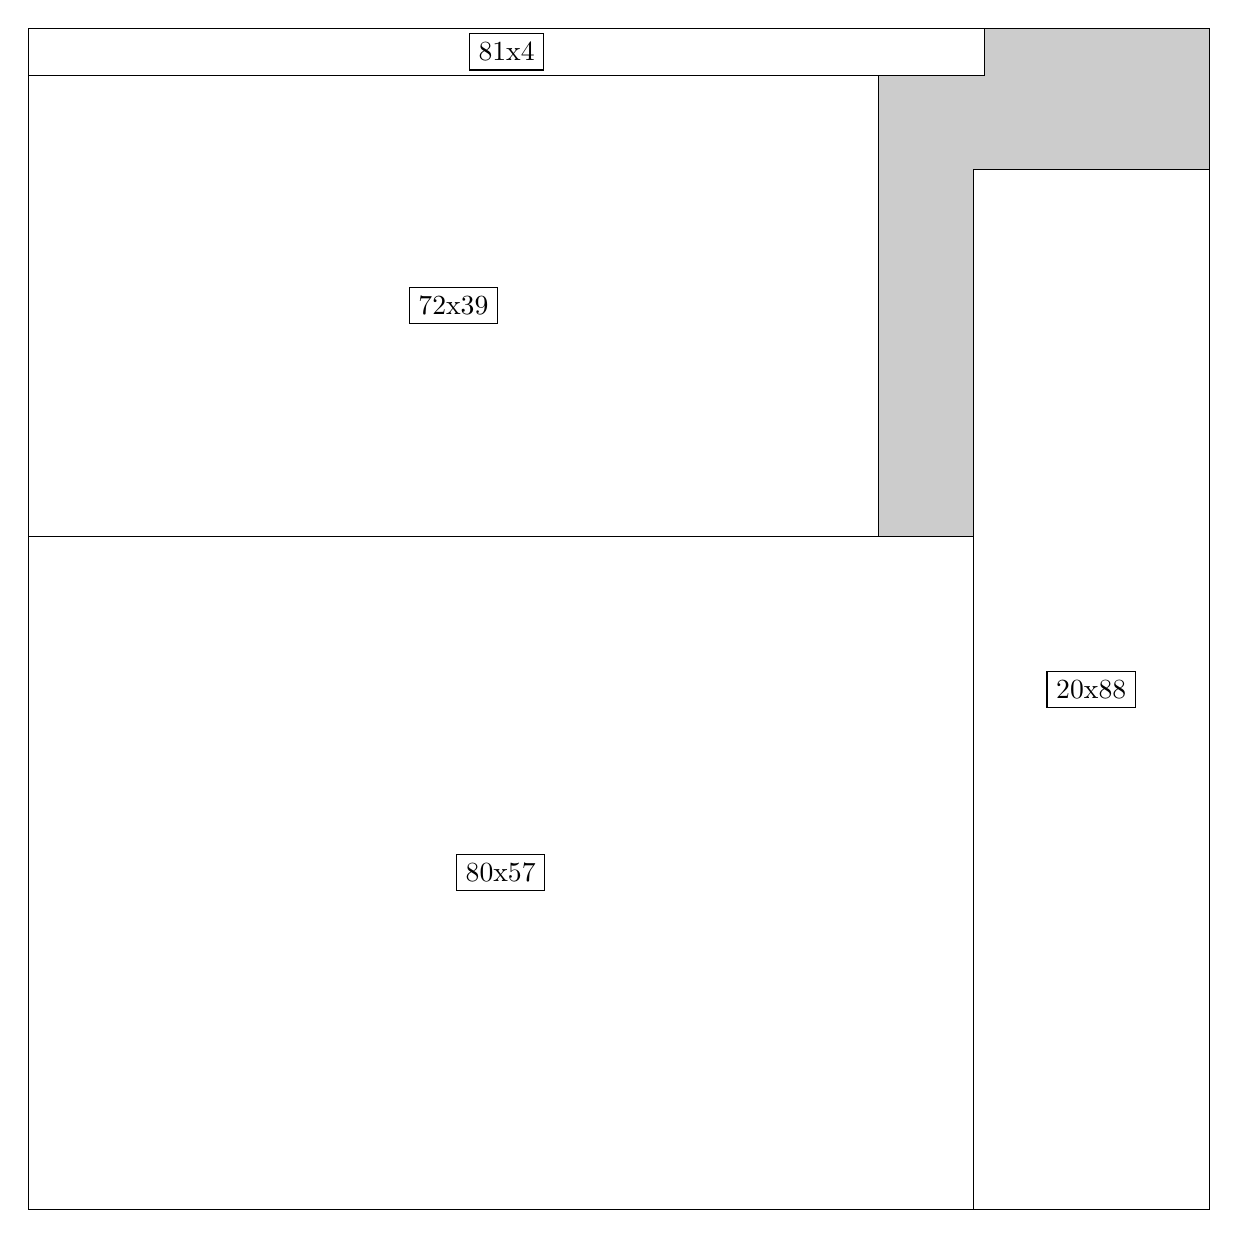
\begin{tikzpicture}[shorten >=1pt,scale=1.0,every node/.style={scale=1.0},->]
\tikzstyle{vertex}=[circle,fill=black!25,minimum size=14pt,inner sep=0pt]
\filldraw[fill=gray!40!white, draw=black] (0,0) rectangle (15.0,15.0);
\foreach \name/\x/\y/\w/\h in {80x57/0.0/0.0/12.0/8.549999999999999,72x39/0.0/8.549999999999999/10.799999999999999/5.85,20x88/12.0/0.0/3.0/13.2,81x4/0.0/14.399999999999999/12.15/0.6}
\filldraw[fill=white!40!white, draw=black] (\x,\y) rectangle node[draw] (\name) {\name} ++(\w,\h);
\end{tikzpicture}


w =80 , h =57 , x =0 , y =0 , v =4560
\par
w =72 , h =39 , x =0 , y =57 , v =2808
\par
w =20 , h =88 , x =80 , y =0 , v =1760
\par
w =81 , h =4 , x =0 , y =96 , v =324
\par
\newpage


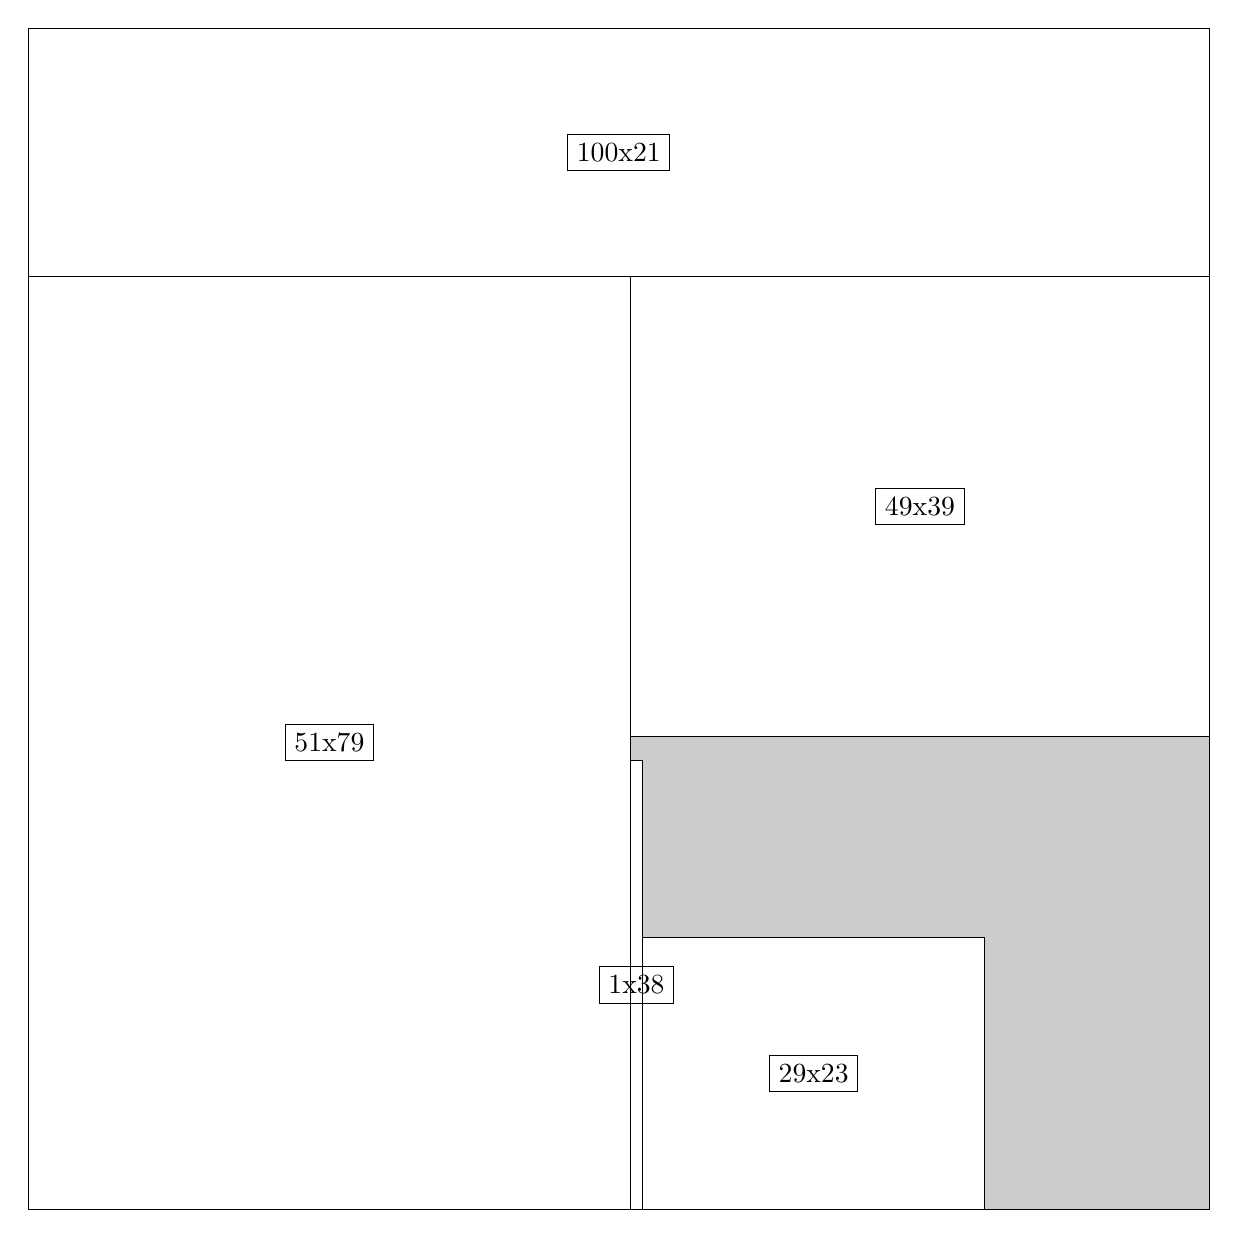
\begin{tikzpicture}[shorten >=1pt,scale=1.0,every node/.style={scale=1.0},->]
\tikzstyle{vertex}=[circle,fill=black!25,minimum size=14pt,inner sep=0pt]
\filldraw[fill=gray!40!white, draw=black] (0,0) rectangle (15.0,15.0);
\foreach \name/\x/\y/\w/\h in {100x21/0.0/11.85/15.0/3.15,49x39/7.6499999999999995/6.0/7.35/5.85,51x79/0.0/0.0/7.6499999999999995/11.85,29x23/7.8/0.0/4.35/3.4499999999999997,1x38/7.6499999999999995/0.0/0.15/5.7}
\filldraw[fill=white!40!white, draw=black] (\x,\y) rectangle node[draw] (\name) {\name} ++(\w,\h);
\end{tikzpicture}


w =100 , h =21 , x =0 , y =79 , v =2100
\par
w =49 , h =39 , x =51 , y =40 , v =1911
\par
w =51 , h =79 , x =0 , y =0 , v =4029
\par
w =29 , h =23 , x =52 , y =0 , v =667
\par
w =1 , h =38 , x =51 , y =0 , v =38
\par
\newpage


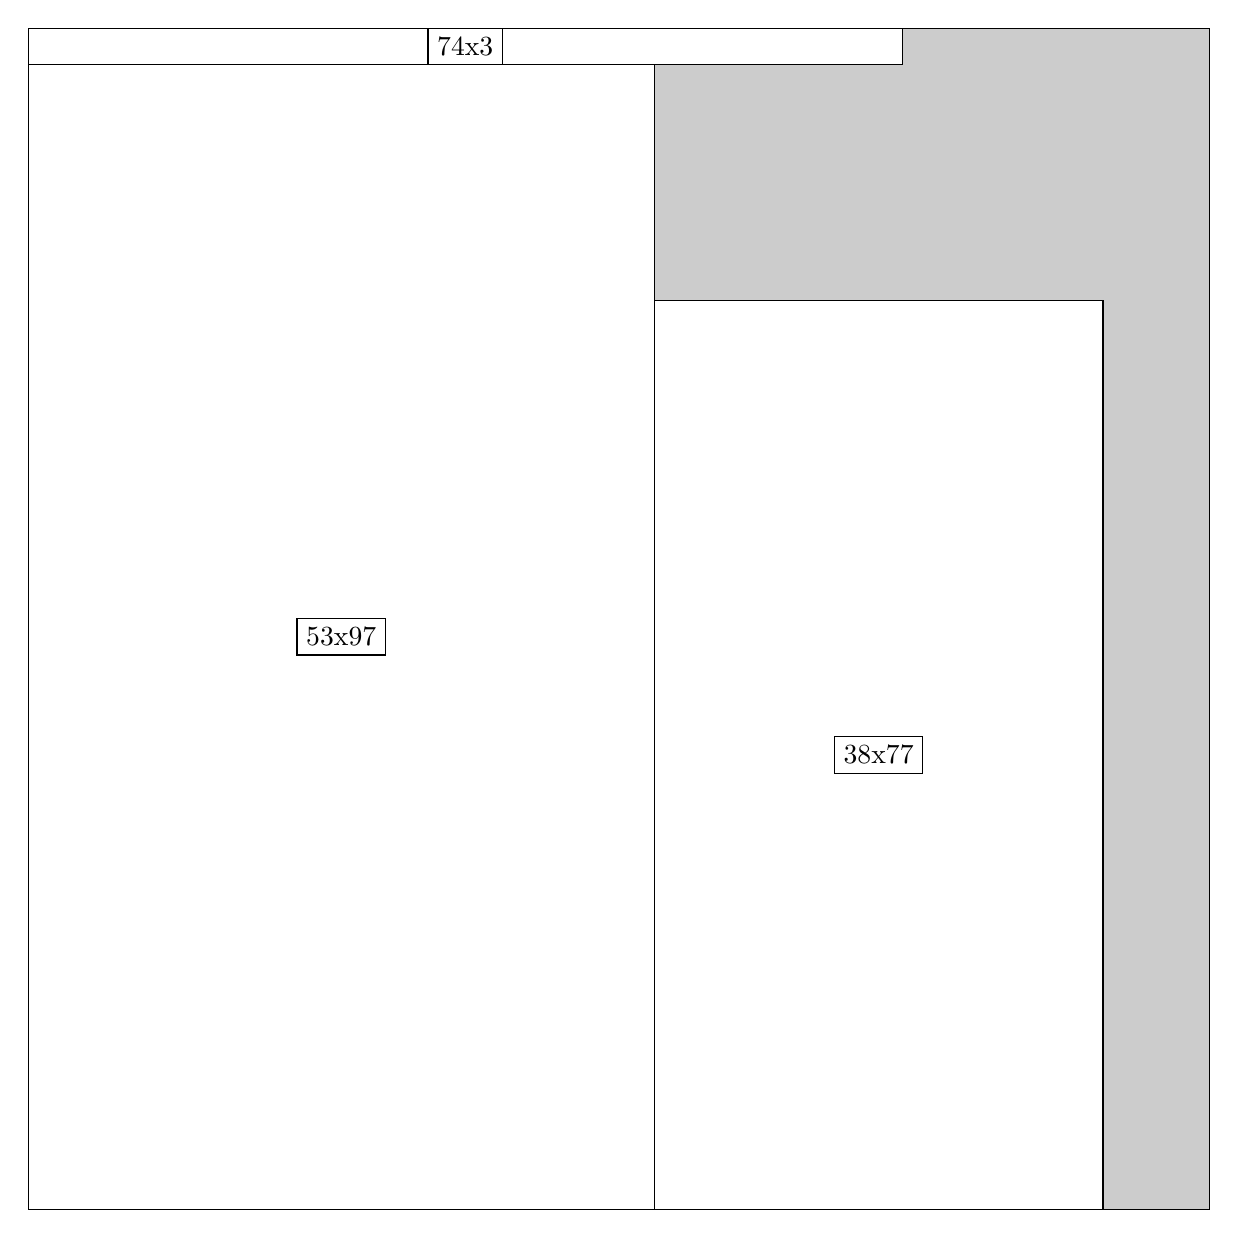
\begin{tikzpicture}[shorten >=1pt,scale=1.0,every node/.style={scale=1.0},->]
\tikzstyle{vertex}=[circle,fill=black!25,minimum size=14pt,inner sep=0pt]
\filldraw[fill=gray!40!white, draw=black] (0,0) rectangle (15.0,15.0);
\foreach \name/\x/\y/\w/\h in {74x3/0.0/14.549999999999999/11.1/0.44999999999999996,38x77/7.949999999999999/0.0/5.7/11.549999999999999,53x97/0.0/0.0/7.949999999999999/14.549999999999999}
\filldraw[fill=white!40!white, draw=black] (\x,\y) rectangle node[draw] (\name) {\name} ++(\w,\h);
\end{tikzpicture}


w =74 , h =3 , x =0 , y =97 , v =222
\par
w =38 , h =77 , x =53 , y =0 , v =2926
\par
w =53 , h =97 , x =0 , y =0 , v =5141
\par
\newpage


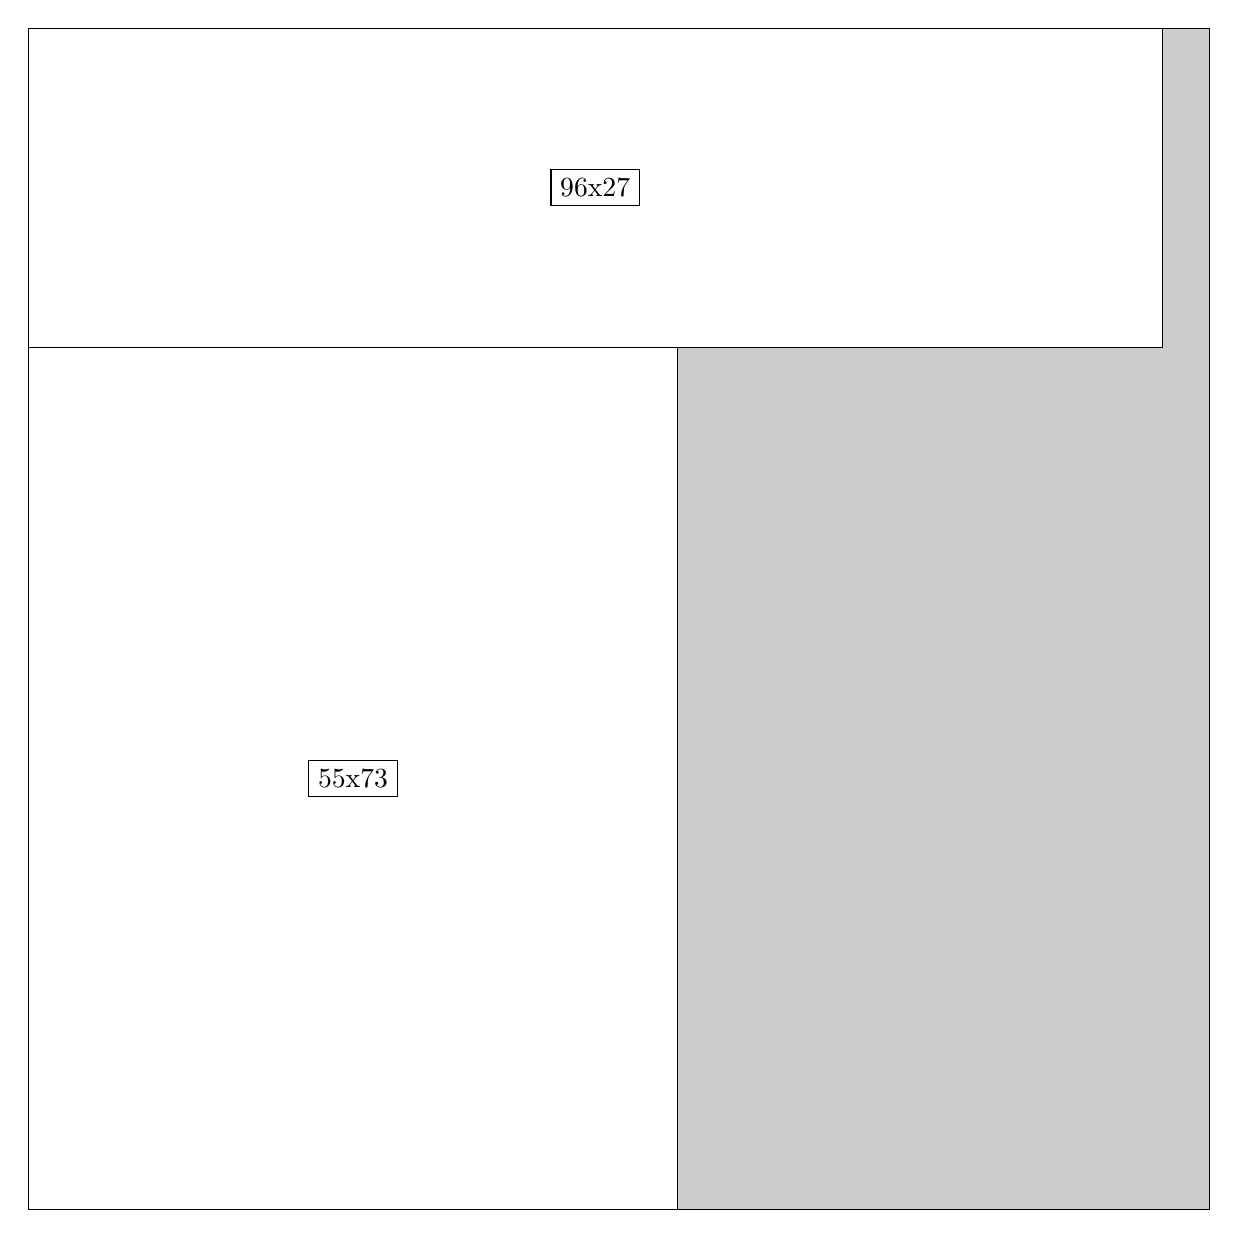
\begin{tikzpicture}[shorten >=1pt,scale=1.0,every node/.style={scale=1.0},->]
\tikzstyle{vertex}=[circle,fill=black!25,minimum size=14pt,inner sep=0pt]
\filldraw[fill=gray!40!white, draw=black] (0,0) rectangle (15.0,15.0);
\foreach \name/\x/\y/\w/\h in {96x27/0.0/10.95/14.399999999999999/4.05,55x73/0.0/0.0/8.25/10.95}
\filldraw[fill=white!40!white, draw=black] (\x,\y) rectangle node[draw] (\name) {\name} ++(\w,\h);
\end{tikzpicture}


w =96 , h =27 , x =0 , y =73 , v =2592
\par
w =55 , h =73 , x =0 , y =0 , v =4015
\par
\newpage


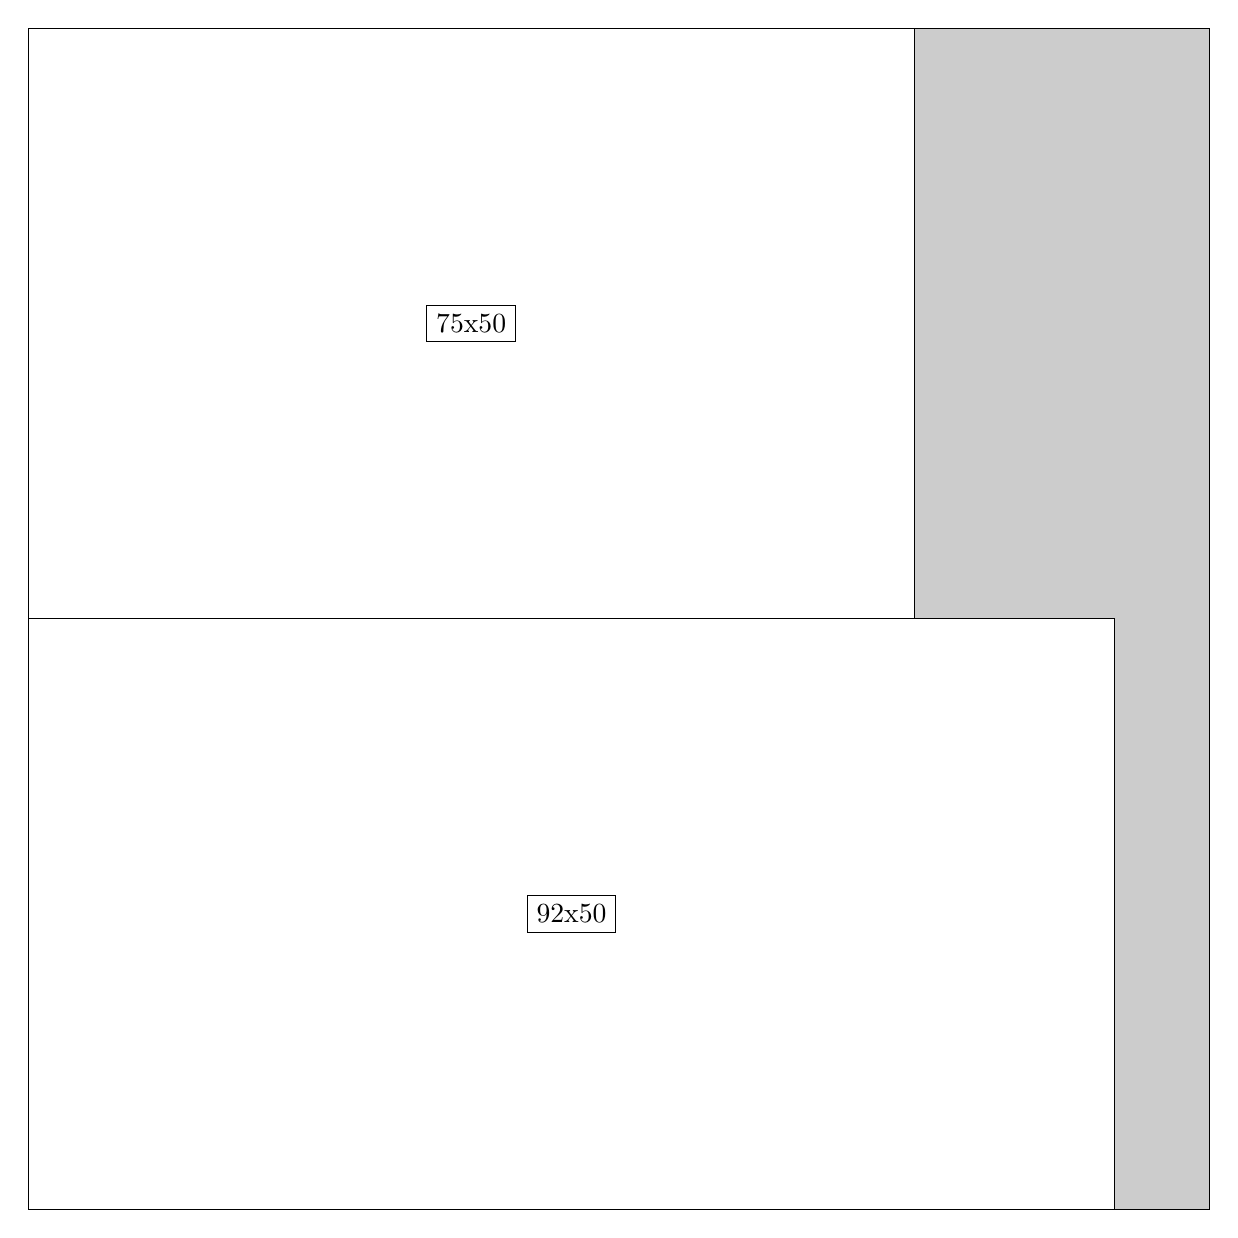
\begin{tikzpicture}[shorten >=1pt,scale=1.0,every node/.style={scale=1.0},->]
\tikzstyle{vertex}=[circle,fill=black!25,minimum size=14pt,inner sep=0pt]
\filldraw[fill=gray!40!white, draw=black] (0,0) rectangle (15.0,15.0);
\foreach \name/\x/\y/\w/\h in {92x50/0.0/0.0/13.799999999999999/7.5,75x50/0.0/7.5/11.25/7.5}
\filldraw[fill=white!40!white, draw=black] (\x,\y) rectangle node[draw] (\name) {\name} ++(\w,\h);
\end{tikzpicture}


w =92 , h =50 , x =0 , y =0 , v =4600
\par
w =75 , h =50 , x =0 , y =50 , v =3750
\par
\newpage


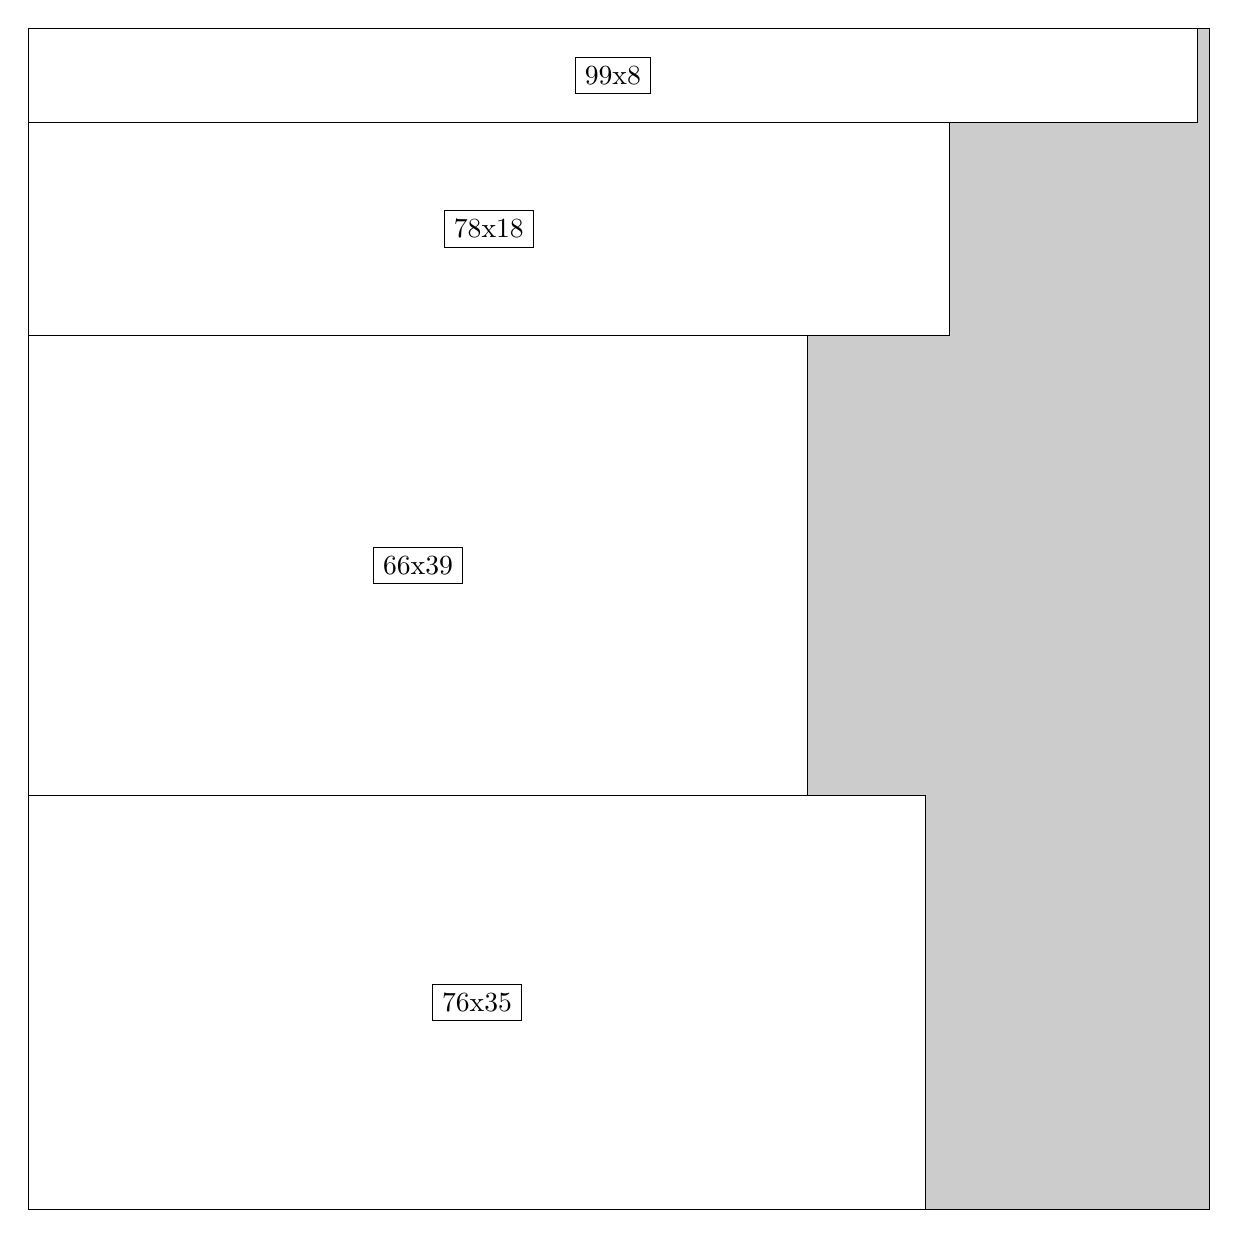
\begin{tikzpicture}[shorten >=1pt,scale=1.0,every node/.style={scale=1.0},->]
\tikzstyle{vertex}=[circle,fill=black!25,minimum size=14pt,inner sep=0pt]
\filldraw[fill=gray!40!white, draw=black] (0,0) rectangle (15.0,15.0);
\foreach \name/\x/\y/\w/\h in {76x35/0.0/0.0/11.4/5.25,78x18/0.0/11.1/11.7/2.6999999999999997,99x8/0.0/13.799999999999999/14.85/1.2,66x39/0.0/5.25/9.9/5.85}
\filldraw[fill=white!40!white, draw=black] (\x,\y) rectangle node[draw] (\name) {\name} ++(\w,\h);
\end{tikzpicture}


w =76 , h =35 , x =0 , y =0 , v =2660
\par
w =78 , h =18 , x =0 , y =74 , v =1404
\par
w =99 , h =8 , x =0 , y =92 , v =792
\par
w =66 , h =39 , x =0 , y =35 , v =2574
\par
\newpage


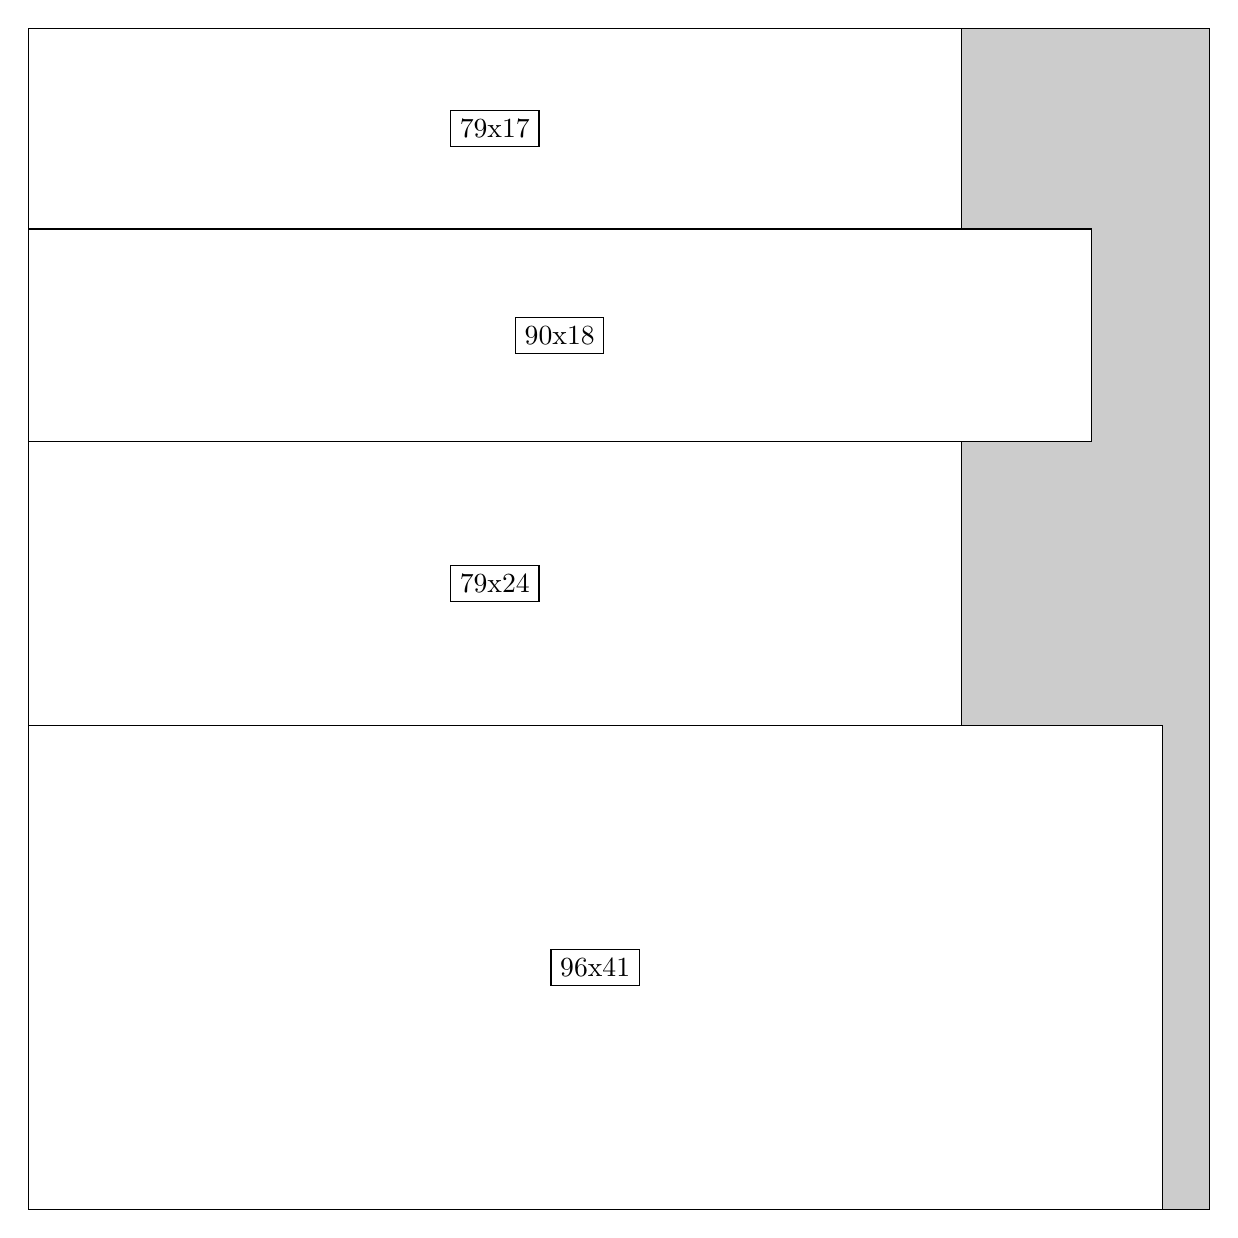
\begin{tikzpicture}[shorten >=1pt,scale=1.0,every node/.style={scale=1.0},->]
\tikzstyle{vertex}=[circle,fill=black!25,minimum size=14pt,inner sep=0pt]
\filldraw[fill=gray!40!white, draw=black] (0,0) rectangle (15.0,15.0);
\foreach \name/\x/\y/\w/\h in {96x41/0.0/0.0/14.399999999999999/6.1499999999999995,79x24/0.0/6.1499999999999995/11.85/3.5999999999999996,90x18/0.0/9.75/13.5/2.6999999999999997,79x17/0.0/12.45/11.85/2.55}
\filldraw[fill=white!40!white, draw=black] (\x,\y) rectangle node[draw] (\name) {\name} ++(\w,\h);
\end{tikzpicture}


w =96 , h =41 , x =0 , y =0 , v =3936
\par
w =79 , h =24 , x =0 , y =41 , v =1896
\par
w =90 , h =18 , x =0 , y =65 , v =1620
\par
w =79 , h =17 , x =0 , y =83 , v =1343
\par
\newpage


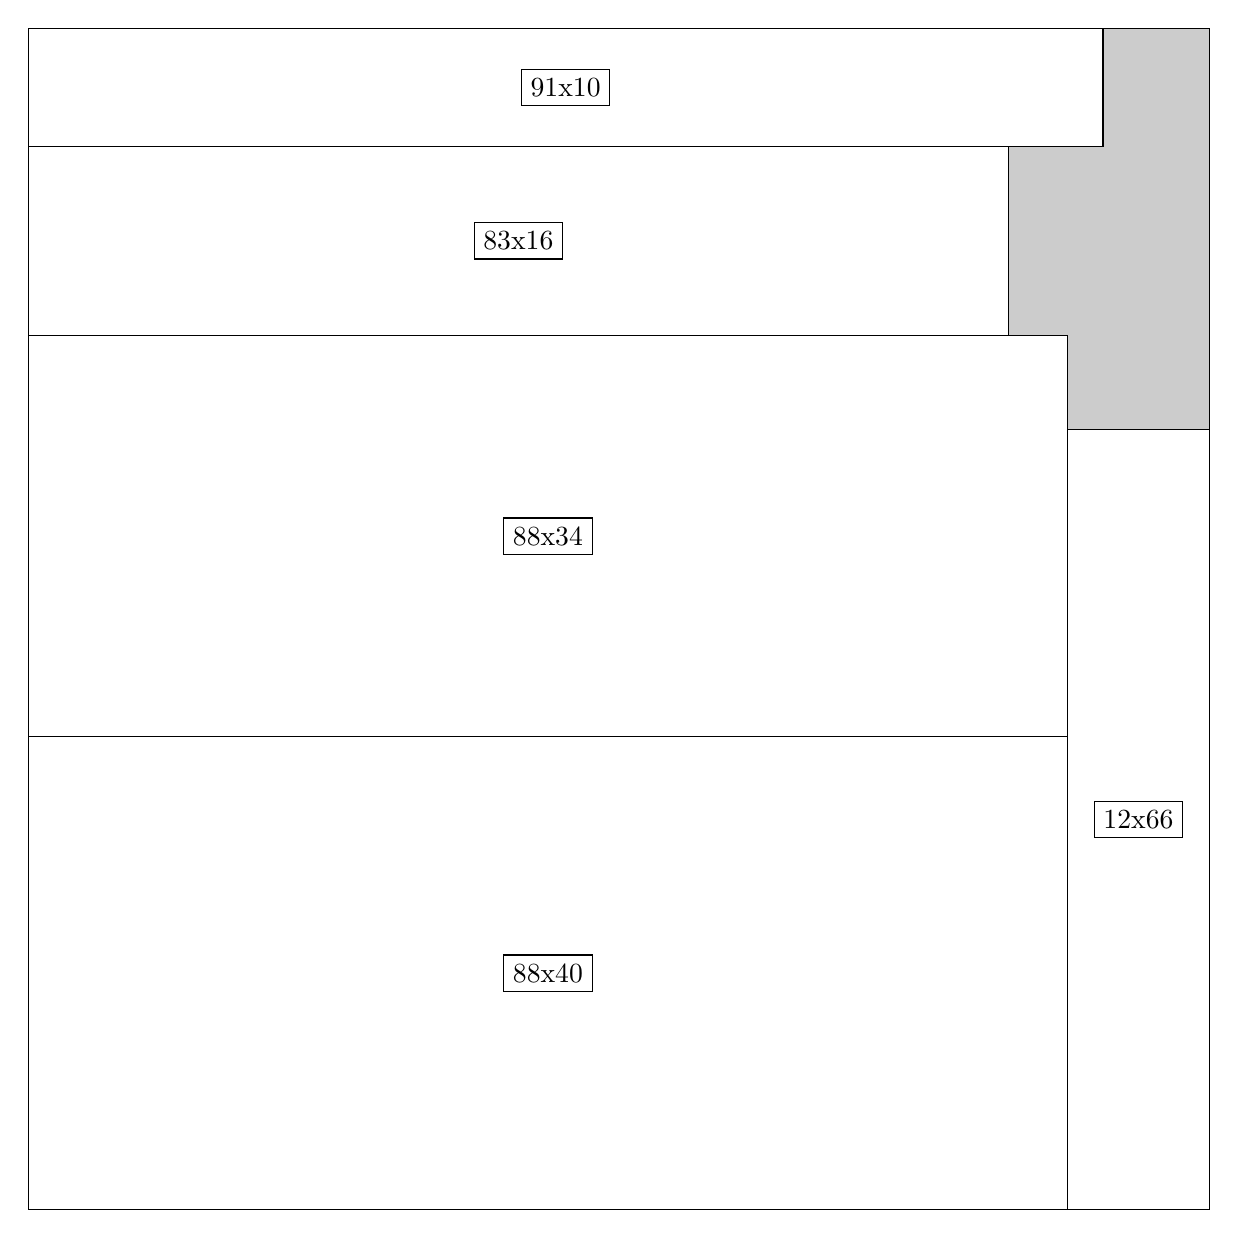
\begin{tikzpicture}[shorten >=1pt,scale=1.0,every node/.style={scale=1.0},->]
\tikzstyle{vertex}=[circle,fill=black!25,minimum size=14pt,inner sep=0pt]
\filldraw[fill=gray!40!white, draw=black] (0,0) rectangle (15.0,15.0);
\foreach \name/\x/\y/\w/\h in {88x40/0.0/0.0/13.2/6.0,88x34/0.0/6.0/13.2/5.1,91x10/0.0/13.5/13.65/1.5,12x66/13.2/0.0/1.7999999999999998/9.9,83x16/0.0/11.1/12.45/2.4}
\filldraw[fill=white!40!white, draw=black] (\x,\y) rectangle node[draw] (\name) {\name} ++(\w,\h);
\end{tikzpicture}


w =88 , h =40 , x =0 , y =0 , v =3520
\par
w =88 , h =34 , x =0 , y =40 , v =2992
\par
w =91 , h =10 , x =0 , y =90 , v =910
\par
w =12 , h =66 , x =88 , y =0 , v =792
\par
w =83 , h =16 , x =0 , y =74 , v =1328
\par
\newpage


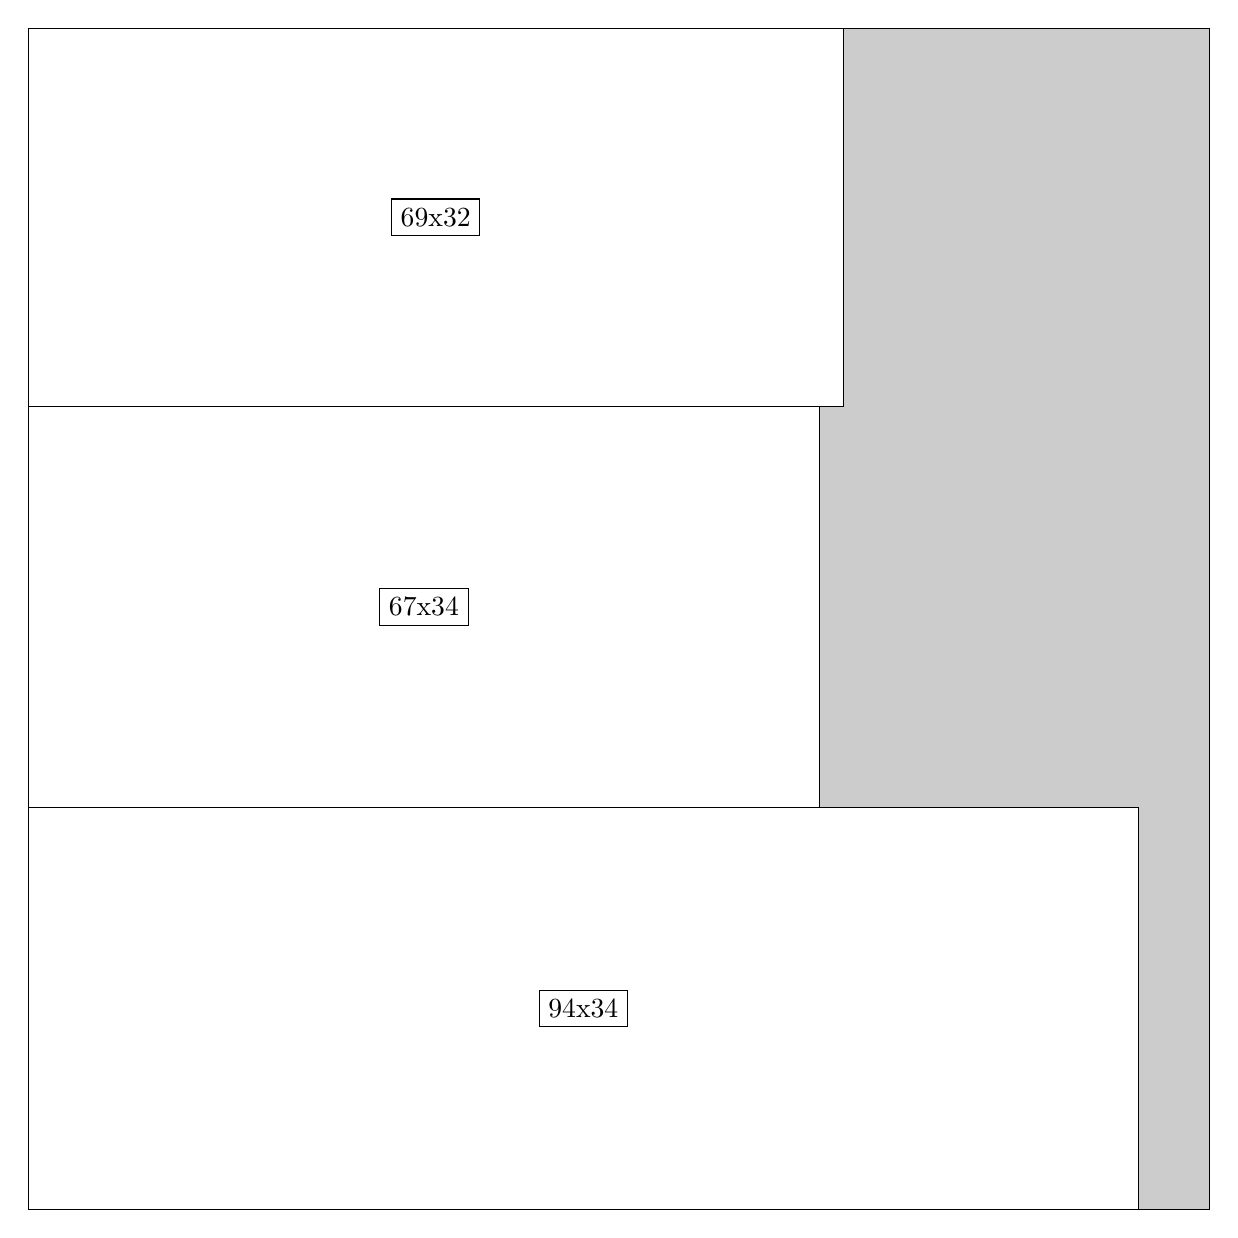
\begin{tikzpicture}[shorten >=1pt,scale=1.0,every node/.style={scale=1.0},->]
\tikzstyle{vertex}=[circle,fill=black!25,minimum size=14pt,inner sep=0pt]
\filldraw[fill=gray!40!white, draw=black] (0,0) rectangle (15.0,15.0);
\foreach \name/\x/\y/\w/\h in {94x34/0.0/0.0/14.1/5.1,67x34/0.0/5.1/10.049999999999999/5.1,69x32/0.0/10.2/10.35/4.8}
\filldraw[fill=white!40!white, draw=black] (\x,\y) rectangle node[draw] (\name) {\name} ++(\w,\h);
\end{tikzpicture}


w =94 , h =34 , x =0 , y =0 , v =3196
\par
w =67 , h =34 , x =0 , y =34 , v =2278
\par
w =69 , h =32 , x =0 , y =68 , v =2208
\par
\newpage


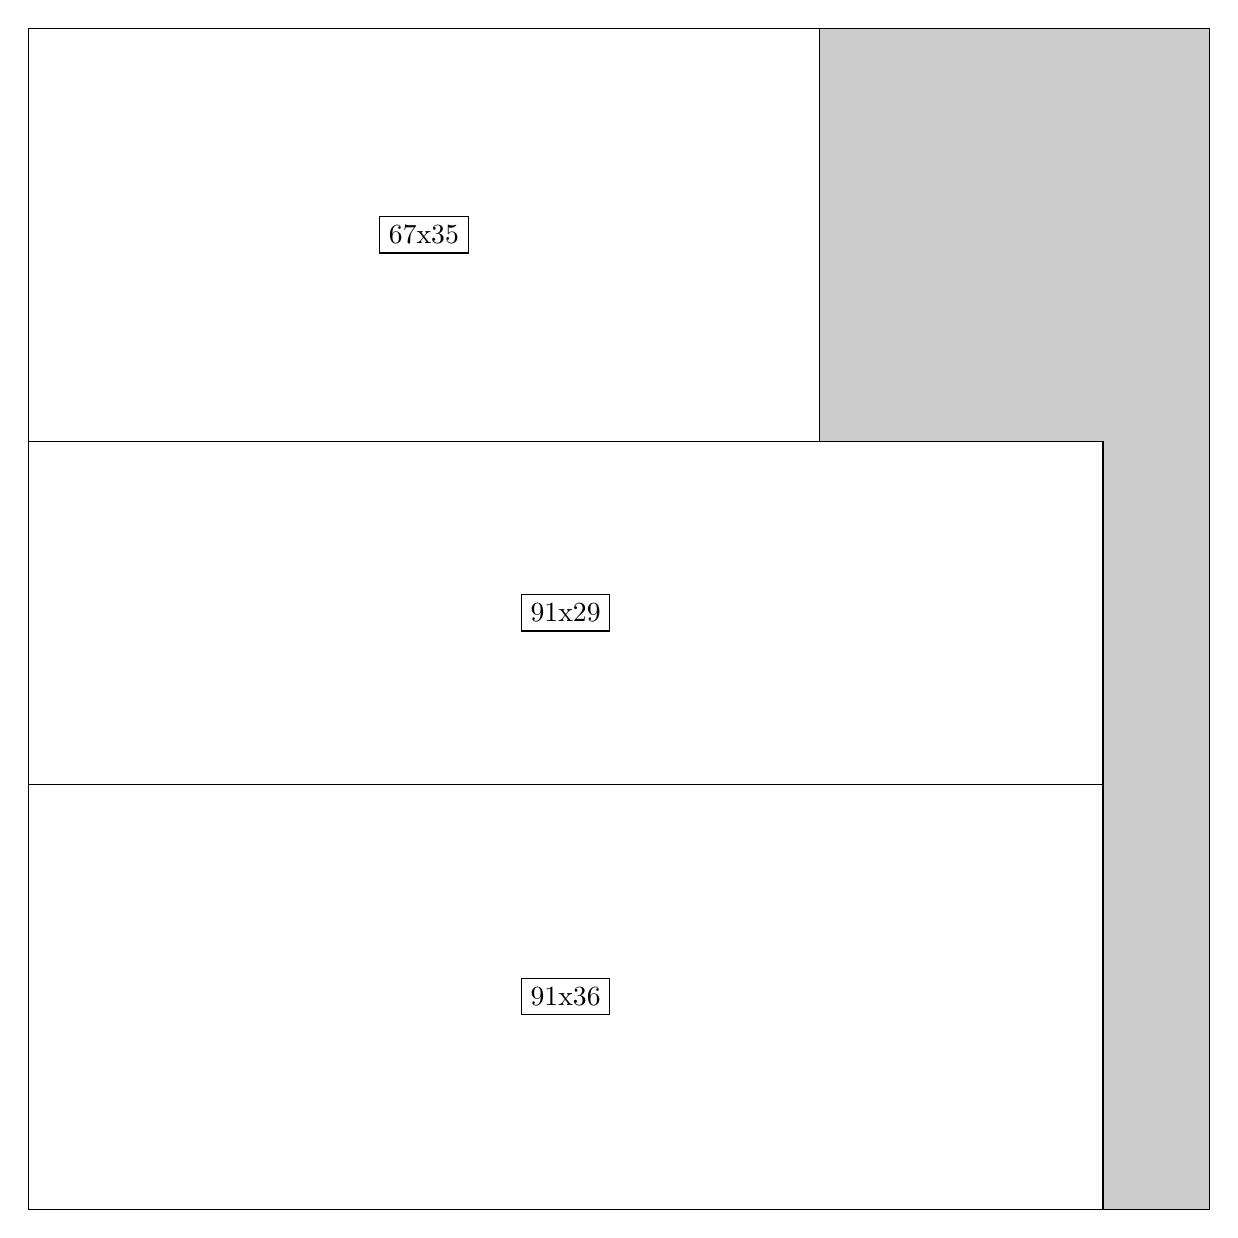
\begin{tikzpicture}[shorten >=1pt,scale=1.0,every node/.style={scale=1.0},->]
\tikzstyle{vertex}=[circle,fill=black!25,minimum size=14pt,inner sep=0pt]
\filldraw[fill=gray!40!white, draw=black] (0,0) rectangle (15.0,15.0);
\foreach \name/\x/\y/\w/\h in {91x36/0.0/0.0/13.65/5.3999999999999995,91x29/0.0/5.3999999999999995/13.65/4.35,67x35/0.0/9.75/10.049999999999999/5.25}
\filldraw[fill=white!40!white, draw=black] (\x,\y) rectangle node[draw] (\name) {\name} ++(\w,\h);
\end{tikzpicture}


w =91 , h =36 , x =0 , y =0 , v =3276
\par
w =91 , h =29 , x =0 , y =36 , v =2639
\par
w =67 , h =35 , x =0 , y =65 , v =2345
\par
\newpage


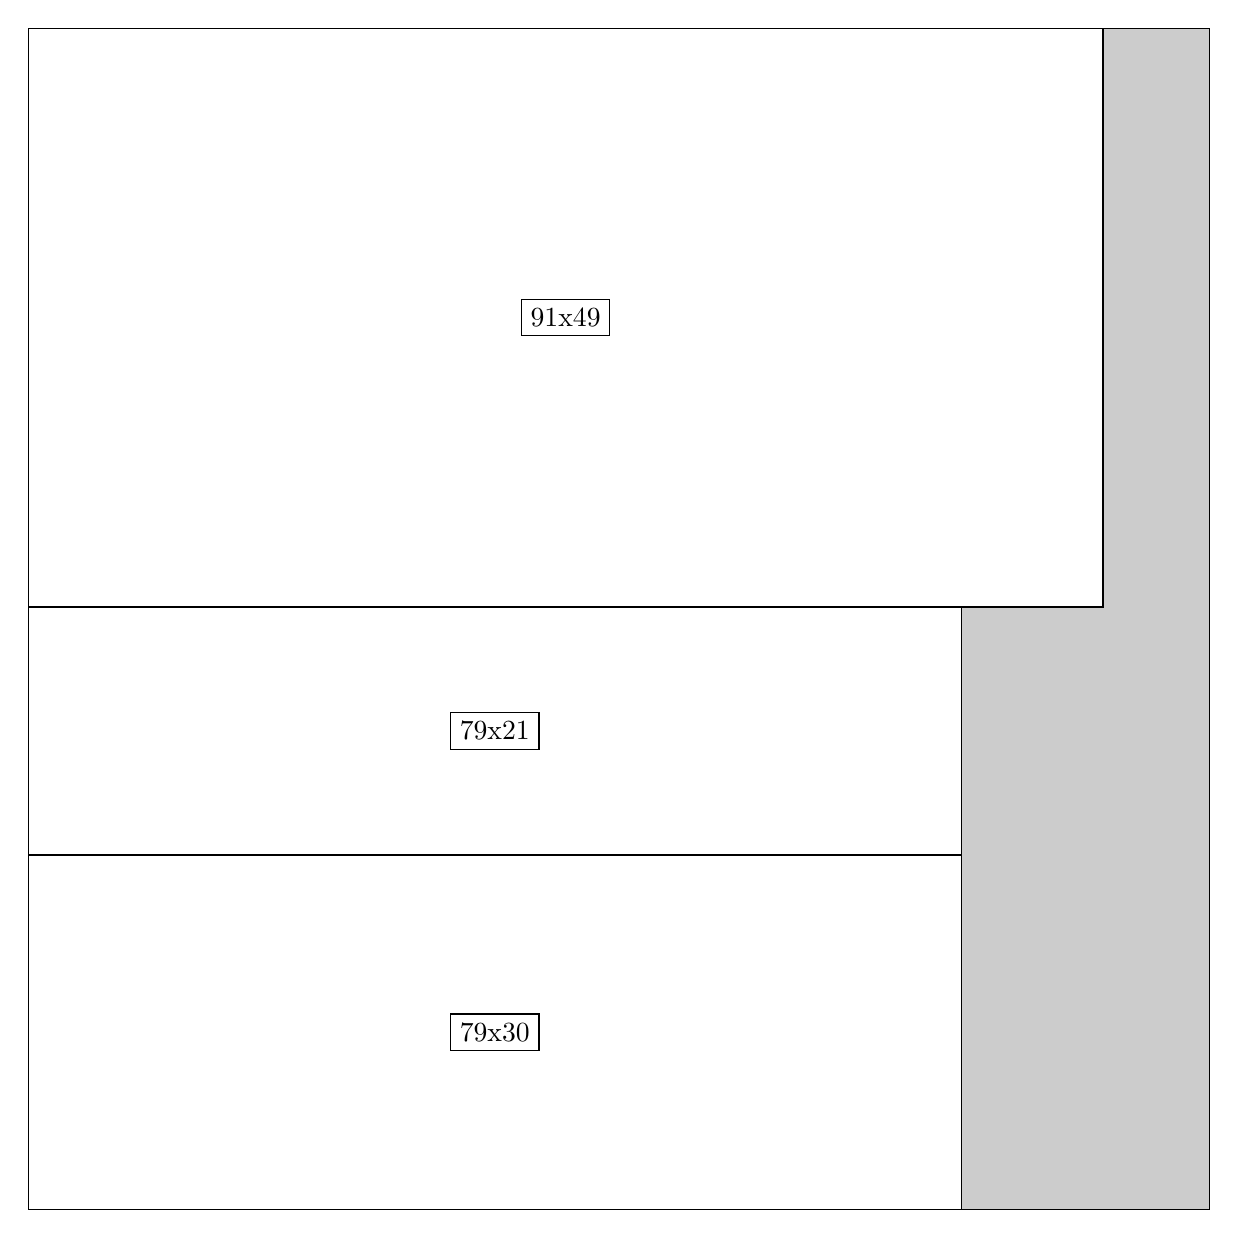
\begin{tikzpicture}[shorten >=1pt,scale=1.0,every node/.style={scale=1.0},->]
\tikzstyle{vertex}=[circle,fill=black!25,minimum size=14pt,inner sep=0pt]
\filldraw[fill=gray!40!white, draw=black] (0,0) rectangle (15.0,15.0);
\foreach \name/\x/\y/\w/\h in {79x30/0.0/0.0/11.85/4.5,91x49/0.0/7.6499999999999995/13.65/7.35,79x21/0.0/4.5/11.85/3.15}
\filldraw[fill=white!40!white, draw=black] (\x,\y) rectangle node[draw] (\name) {\name} ++(\w,\h);
\end{tikzpicture}


w =79 , h =30 , x =0 , y =0 , v =2370
\par
w =91 , h =49 , x =0 , y =51 , v =4459
\par
w =79 , h =21 , x =0 , y =30 , v =1659
\par
\newpage


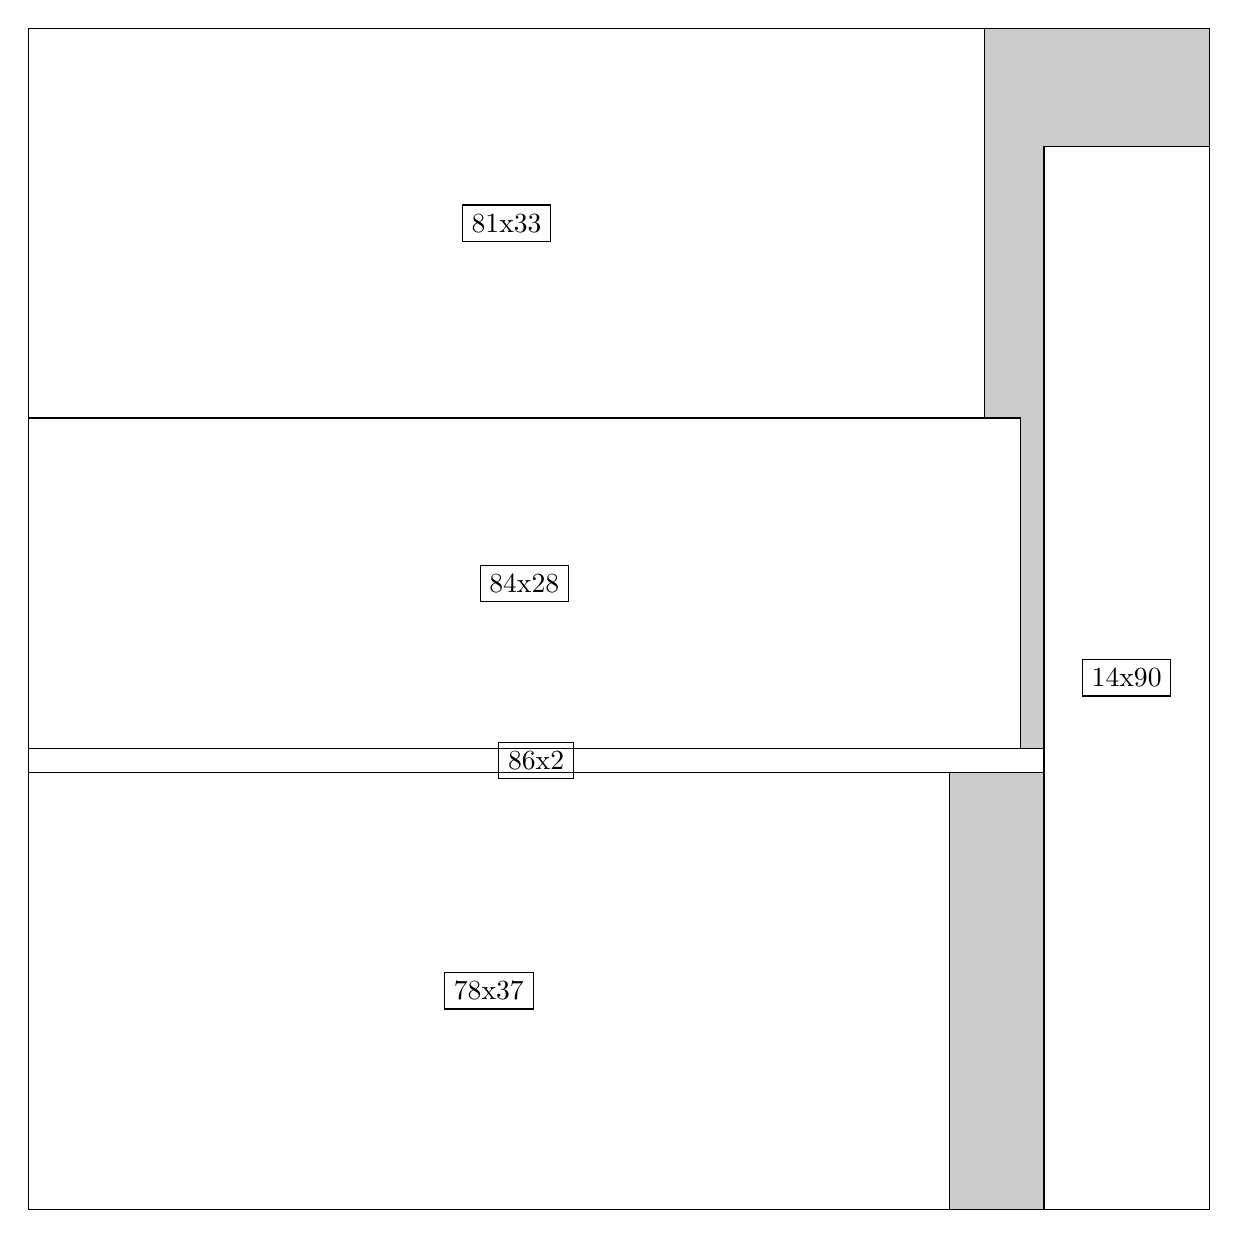
\begin{tikzpicture}[shorten >=1pt,scale=1.0,every node/.style={scale=1.0},->]
\tikzstyle{vertex}=[circle,fill=black!25,minimum size=14pt,inner sep=0pt]
\filldraw[fill=gray!40!white, draw=black] (0,0) rectangle (15.0,15.0);
\foreach \name/\x/\y/\w/\h in {78x37/0.0/0.0/11.7/5.55,81x33/0.0/10.049999999999999/12.15/4.95,84x28/0.0/5.85/12.6/4.2,14x90/12.9/0.0/2.1/13.5,86x2/0.0/5.55/12.9/0.3}
\filldraw[fill=white!40!white, draw=black] (\x,\y) rectangle node[draw] (\name) {\name} ++(\w,\h);
\end{tikzpicture}


w =78 , h =37 , x =0 , y =0 , v =2886
\par
w =81 , h =33 , x =0 , y =67 , v =2673
\par
w =84 , h =28 , x =0 , y =39 , v =2352
\par
w =14 , h =90 , x =86 , y =0 , v =1260
\par
w =86 , h =2 , x =0 , y =37 , v =172
\par
\newpage


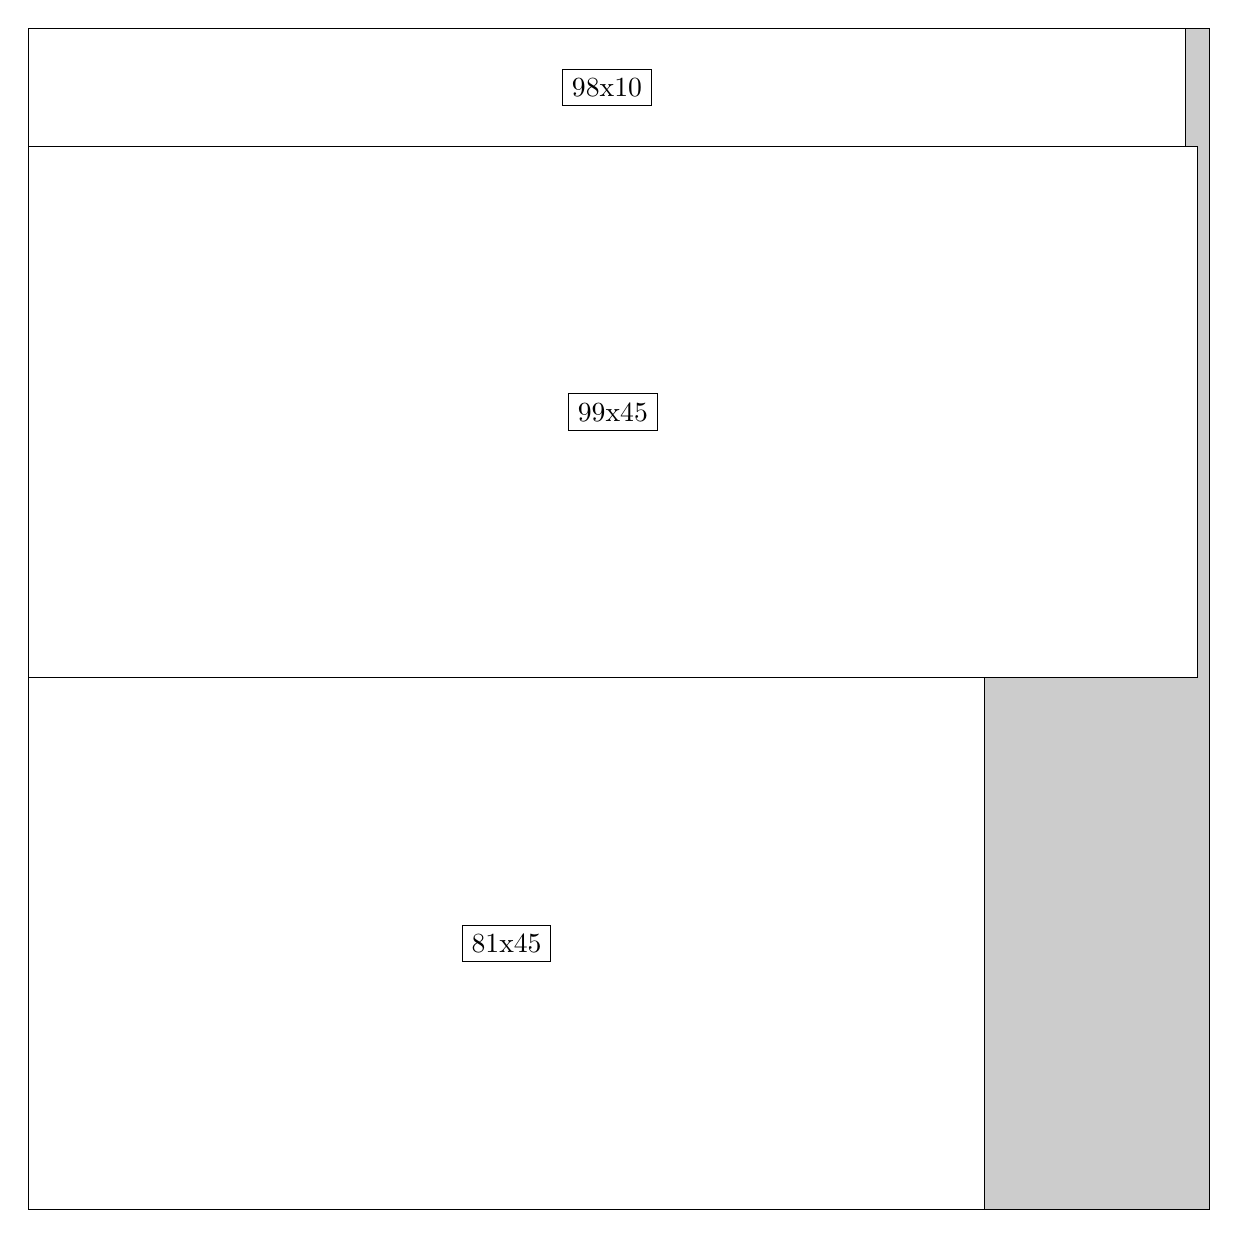
\begin{tikzpicture}[shorten >=1pt,scale=1.0,every node/.style={scale=1.0},->]
\tikzstyle{vertex}=[circle,fill=black!25,minimum size=14pt,inner sep=0pt]
\filldraw[fill=gray!40!white, draw=black] (0,0) rectangle (15.0,15.0);
\foreach \name/\x/\y/\w/\h in {81x45/0.0/0.0/12.15/6.75,99x45/0.0/6.75/14.85/6.75,98x10/0.0/13.5/14.7/1.5}
\filldraw[fill=white!40!white, draw=black] (\x,\y) rectangle node[draw] (\name) {\name} ++(\w,\h);
\end{tikzpicture}


w =81 , h =45 , x =0 , y =0 , v =3645
\par
w =99 , h =45 , x =0 , y =45 , v =4455
\par
w =98 , h =10 , x =0 , y =90 , v =980
\par
\newpage


\end{document}